\section{P3C-Orch Framework}
Fig.~\ref{fig:system_model} shows the \pchorch\ system model. The controller receives mobility, cache, load, energy, and link states from the UAV swarms and demand clusters. It predicts next-slot link margin, estimates outage risk, computes cache value, applies dwell control, and assigns each active demand cluster to a feasible swarm.

\begin{figure}[!t]
\centering
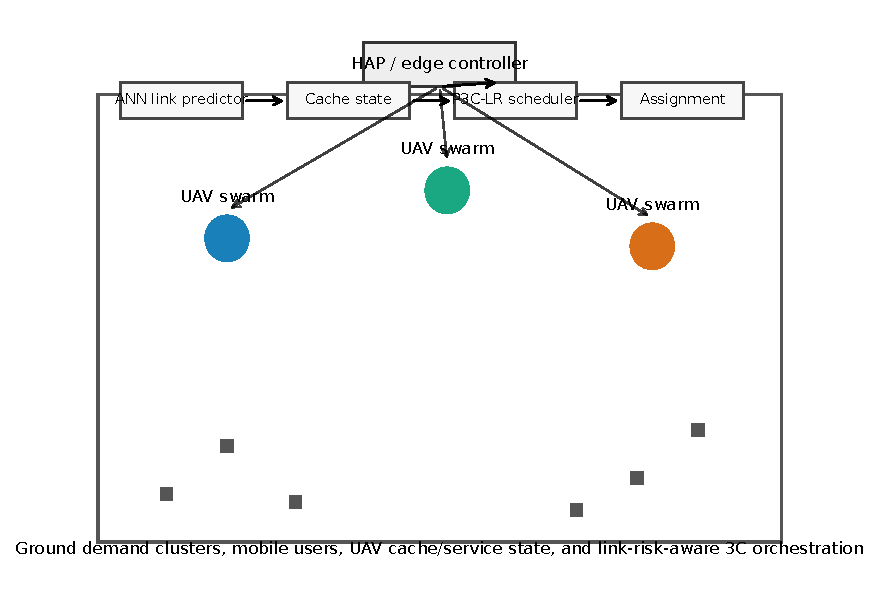
\includegraphics[width=\columnwidth]{figs/system_model_p3clr.pdf}
\caption{System model of \pchorch. Ground users generate content requests, UAV swarms provide service and cache reuse, and the edge controller uses link prediction, cache state, and scheduling state for assignment.}
\label{fig:system_model}
\end{figure}

\begin{figure}[!t]
\centering
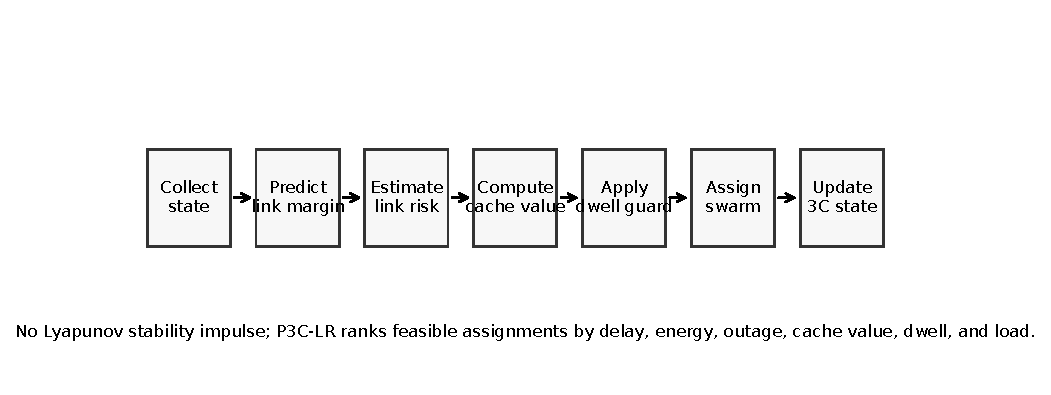
\includegraphics[width=\columnwidth]{figs/algorithm_flow_p3clr.pdf}
\caption{Algorithm flow of \pchorch. The controller collects state, predicts link risk, computes cache value and dwell cost, assigns swarms, and updates queue, cache, energy, and handover states.}
\label{fig:algorithm_flow}
\end{figure}

For \pclr, every feasible swarm-cluster pair receives a normalized score:
\begin{align}
B_{s,k,t}={}&w_m\norm{m}_{s,k,t}+w_c\norm{V}^{\mathrm{cache}}_{s,k,t}+w_f\norm{F}_{s,t}+w_r\norm{R}^{\mathrm{dwell}}_{s,k,t}\nonumber\\
&-w_d\norm{D}_{s,k,t}-w_e\norm{C}^{\mathrm{en}}_{s,k,t}-w_o\norm{p}^{\mathrm{out}}_{s,k,t}\nonumber\\
&-w_h\norm{C}^{\mathrm{sw}}_{s,k,t}-w_l\norm{L}_{s,t}.
\label{eq:p3clr_score}
\end{align}
Here, $\norm{m}$ is the normalized risk-adjusted link margin, $\norm{V}^{\mathrm{cache}}$ is normalized useful cache value, $\norm{F}$ is a fairness term, $\norm{R}^{\mathrm{dwell}}$ rewards staying with the previous feasible swarm, $\norm{D}$ is delay cost, $\norm{C}^{\mathrm{en}}$ is energy cost, $\norm{p}^{\mathrm{out}}$ is outage risk, $\norm{C}^{\mathrm{sw}}$ is switching cost, and $\norm{L}$ is swarm load. The normalization is done per slot over feasible pairs so that no single raw scale dominates the score.

The scheduling problem is
\begin{align}
\max_{x_{s,k,t}} &\quad \sum_{k\in\mathcal{K}_t}\sum_{s\in\mathcal{S}} x_{s,k,t}B_{s,k,t} \label{eq:assignment_problem}\\
\mathrm{s.t.} &\quad \sum_s x_{s,k,t}\leq 1,\quad \forall k,\nonumber\\
&\quad \sum_k x_{s,k,t}\mu_{s,k,t}\leq \bar{\mu}_{s,t},\quad \forall s,\nonumber\\
&\quad x_{s,k,t}\in\{0,1\}.\nonumber
\end{align}
The implementation uses greedy assignment ordered by deadline-aware urgency and backlog for scalability. A dwell guard keeps the previous swarm if it remains feasible and if the new score gain is too small to justify a handover. This guard is important because KMeans-like cluster movement can otherwise create unnecessary handovers.

The paper objective is used only for ranking the final results, not for tuning on paper-lock seeds:
\begin{align}
J={}&0.18\norm{D}_{\mathrm{avg}}+0.16\norm{D}_{95}+0.16\norm{E}+0.14\norm{H}\nonumber\\
&+0.12\norm{p}^{\mathrm{out}}+0.10\norm{P}_{\mathrm{drop}}+0.08\norm{I}_{\mathrm{load}}\nonumber\\
&-0.08\norm{H}^{\mathrm{cache}}-0.08\norm{T}_{\mathrm{put}}-0.04\norm{F}_{\mathrm{Jain}}.
\label{eq:paper_objective}
\end{align}
A lower value of $J$ is better. Individual metrics are always reported with the objective.
